% Gabarit pandoc des corrigés publiés (brut et guidé). Contenu sans marque ni nom de site.
% Compilation : lualatex (latexmk -lualatex).
% Le Markdown reste la source unique : ne pas éditer ce fichier .tex à la main.
\documentclass[11pt,a4paper]{article}

% --- Moteur, polices (Latin Modern) et langue ---------------------------------
\usepackage{iftex}
\ifLuaTeX\else\errmessage{Ce document se compile avec lualatex}\fi
\usepackage{amsmath,amssymb,mathtools}
\usepackage{fontspec}
% mathrm=sym : \mathrm prend ses glyphes dans la police mathématique (ℓ, μ, Ω), comme KaTeX.
\usepackage[math-style=TeX,bold-style=TeX,mathrm=sym]{unicode-math}
% Repli pour les glyphes absents de Latin Modern (indices et exposants Unicode,
% flèches, filets des schémas en texte, symboles) : DejaVu, puis Latin Modern Math
% (ℓ, lettres mathématiques Unicode des légendes).
\directlua{
  luaotfload.add_fallback("repliTexte", {"DejaVuSerif:mode=harf;", "DejaVuSans:mode=harf;", "file:latinmodern-math.otf:mode=harf;"})
  luaotfload.add_fallback("repliMono", {"DejaVuSansMono:mode=harf;", "DejaVuSans:mode=harf;", "file:latinmodern-math.otf:mode=harf;"})
}
\setmainfont{Latin Modern Roman}[RawFeature={fallback=repliTexte}]
\setsansfont{Latin Modern Sans}[RawFeature={fallback=repliTexte}]
\setmonofont{Latin Modern Mono}[RawFeature={fallback=repliMono}]
\setmathfont{Latin Modern Math}
\usepackage[french]{babel}
\frenchsetup{SmallCapsFigTabCaptions=false}

% --- Mise en page --------------------------------------------------------------
\usepackage[a4paper,margin=2.2cm,headheight=14pt,footskip=1.2cm]{geometry}
\usepackage{microtype}
\setlength{\emergencystretch}{4em}
\tolerance=1500
\setlength{\parindent}{0pt}
\setlength{\parskip}{0.55\baselineskip plus 2pt minus 1pt}
\usepackage{xcolor}
% Gris nommés : babel-french rend « ! » actif dans le document.
\definecolor{gris2}{gray}{0.98}
\definecolor{gris3}{gray}{0.97}
\definecolor{gris5}{gray}{0.95}
\definecolor{gris35}{gray}{0.65}
\definecolor{gris40}{gray}{0.60}
\definecolor{gris45}{gray}{0.55}
\definecolor{gris50}{gray}{0.50}
\definecolor{gris55}{gray}{0.45}
\definecolor{gris60}{gray}{0.40}
\definecolor{gris65}{gray}{0.35}
\definecolor{gris70}{gray}{0.30}
\definecolor{gris80}{gray}{0.20}
\definecolor{gris85}{gray}{0.15}
\usepackage{graphicx}
\usepackage{float}
\usepackage{caption}
\captionsetup{font=small,labelformat=empty,justification=centering}
\usepackage{booktabs,longtable,array,multirow,calc}
\usepackage{siunitx}
\sisetup{locale=FR}
\usepackage[version=4]{mhchem}
\usepackage{listings}
\usepackage{fancyhdr}
\usepackage{lastpage}
\usepackage[most]{tcolorbox}
\usepackage{enumitem}
\setlist{nosep,leftmargin=*,topsep=2pt}
\usepackage[hidelinks,unicode]{hyperref}
\usepackage{bookmark}
\hypersetup{pdftitle={ATS — Mathématiques 2026},pdfauthor={Rédigé par IA},pdfcreator={LaTeX},pdfsubject={Corrigé brut}}
\usepackage{xurl}

% --- Pandoc : listes, tableaux, figures ----------------------------------------
\providecommand{\passthrough}[1]{#1}
\providecommand{\tightlist}{\setlength{\itemsep}{0pt}\setlength{\parskip}{0pt}}

\makeatletter
\def\maxwidth{\ifdim\Gin@nat@width>\linewidth\linewidth\else\Gin@nat@width\fi}
\def\maxheight{\ifdim\Gin@nat@height>0.55\textheight 0.55\textheight\else\Gin@nat@height\fi}
\makeatother
\setkeys{Gin}{width=\maxwidth,height=\maxheight,keepaspectratio}
\setcounter{secnumdepth}{-\maxdimen}
\providecommand{\pandocbounded}[1]{#1}
\usepackage{longtable,booktabs,array}

% --- Code (listings) -----------------------------------------------------------
\lstset{
  basicstyle=\ttfamily\small,
  columns=fullflexible,
  keepspaces=true,
  breaklines=true,
  breakatwhitespace=false,
  postbreak=\mbox{\textcolor{gris50}{$\hookrightarrow$}\space},
  frame=single,
  rulecolor=\color{gris35},
  framesep=4pt,
  xleftmargin=5pt,xrightmargin=5pt,
  backgroundcolor=\color{gris3},
  keywordstyle=\bfseries,
  commentstyle=\color{gris65},
  stringstyle=\color{gris80},
  showstringspaces=false,
  tabsize=4,
  extendedchars=true,
  aboveskip=6pt,belowskip=6pt,
}

% --- Macros des corrigés (KaTeX ↔ LaTeX) ---------------------------------------
% Les corrigés sont écrits pour KaTeX : on définit ici ce que KaTeX connaît et
% que LaTeX n'a pas, sans jamais retoucher le Markdown.
\providecommand{\R}{\mathbb{R}}
\providecommand{\N}{\mathbb{N}}
\providecommand{\Z}{\mathbb{Z}}
\providecommand{\Q}{\mathbb{Q}}
\providecommand{\C}{\mathbb{C}}
\providecommand{\dd}{\mathrm{d}}
\providecommand{\llbracket}{\lBrack}
\providecommand{\rrbracket}{\rBrack}
\providecommand{\lBrace}{\lbrace}
\providecommand{\rBrace}{\rbrace}
\providecommand{\Box}{\square}
\providecommand{\Diamond}{\lozenge}
\providecommand{\varnothing}{\emptyset}
\providecommand{\argmax}{\operatorname*{arg\,max}}
\providecommand{\argmin}{\operatorname*{arg\,min}}
\renewcommand{\leq}{\leqslant}
\renewcommand{\geq}{\geqslant}

% Équation hors texte : réduite à la largeur de la ligne si elle déborde.
\newsavebox{\boiteequation}
\newcommand{\equationajustee}[1]{%
  \sbox{\boiteequation}{$\displaystyle #1$}%
  \ifdim\wd\boiteequation>\linewidth
    \[\resizebox{\linewidth}{!}{\usebox{\boiteequation}}\]%
  \else
    \[#1\]%
  \fi}

% --- Encadrés pédagogiques (sobres, lisibles en noir et blanc) -----------------
\tcbset{
  encadre/.style={
    enhanced,breakable,sharp corners,
    colback=white,colframe=gris55,
    boxrule=0.4pt,leftrule=2.2pt,
    left=6pt,right=6pt,top=3pt,bottom=3pt,
    before skip=6pt,after skip=6pt,
    fonttitle=\bfseries\small,coltitle=black,
    attach title to upper,after title={\quad},
    parbox=false,
  }
}
\newtcolorbox{indication}[1]{encadre,colframe=gris45,colback=gris2,title={Indication~#1}}
\newtcolorbox{methode}{encadre,colframe=gris70,title={Méthode}}
\newtcolorbox{piege}{encadre,colframe=gris85,boxrule=0.8pt,leftrule=2.2pt,title={Piège}}
\newtcolorbox{jury}{encadre,colframe=gris60,colback=gris5,title={Jury}}
\newtcolorbox{encadrenote}{encadre,colframe=gris40}

% --- Titres de section ---------------------------------------------------------
\usepackage{titlesec}
\titleformat{\section}{\Large\bfseries}{}{0pt}{}
\titleformat{\subsection}{\large\bfseries}{}{0pt}{}
\titleformat{\subsubsection}{\normalsize\bfseries}{}{0pt}{}
\titlespacing*{\section}{0pt}{14pt plus 4pt minus 2pt}{6pt}
\titlespacing*{\subsection}{0pt}{10pt plus 3pt minus 2pt}{4pt}
\titlespacing*{\subsubsection}{0pt}{8pt plus 2pt minus 2pt}{2pt}

% --- En-tête et pied de page ---------------------------------------------------
\pagestyle{fancy}
\fancyhf{}
\fancyhead[L]{\small\textsc{Corrigé brut} · ATS ATS}
\fancyhead[R]{\small Maths 2026}
\fancyfoot[L]{\footnotesize Corrigé rédigé par IA, non officiel}
\fancyfoot[R]{\footnotesize \thepage\,/\,\pageref*{LastPage}}
\renewcommand{\headrulewidth}{0.4pt}
\renewcommand{\footrulewidth}{0pt}
\fancypagestyle{plain}{\fancyhf{}\fancyfoot[R]{\footnotesize \thepage\,/\,\pageref*{LastPage}}\fancyfoot[L]{\footnotesize Corrigé rédigé par IA, non officiel}\renewcommand{\headrulewidth}{0pt}}

\begin{document}
\thispagestyle{plain}
\begin{center}
  {\small\scshape Corrigé brut}\par\smallskip
  {\LARGE\bfseries ATS — Mathématiques 2026\par}\medskip
  {\large ATS · ATS · Maths · 2026\par}
\end{center}
\vspace{2pt}\hrule\vspace{8pt}

\emph{Corrigé rédigé par IA, non officiel. Signalez toute erreur.}

Épreuve de 3 h, calculatrice interdite. Quatre exercices indépendants.

\begin{center}\rule{0.5\linewidth}{0.5pt}\end{center}

\hypertarget{exercice-1}{%
\section{Exercice 1}\label{exercice-1}}

Notations : \(f\) est \(2\pi\)-périodique et impaire, avec \(f(t)=\frac{\pi-t}{2}\) sur \(]0,\pi[\) et \(f(0)=0\).

Coefficients de Fourier, avec la convention \(S(t)=a_0+\sum_{k\ge1}(a_k\cos(kt)+b_k\sin(kt))\) :

\equationajustee{\begin{aligned}
a_0&=\frac{1}{2\pi}\int_{-\pi}^{\pi}f(t)\,dt,\\
a_n&=\frac1\pi\int_{-\pi}^{\pi}f(t)\cos(nt)\,dt\quad(n\ge1),\\
b_n&=\frac1\pi\int_{-\pi}^{\pi}f(t)\sin(nt)\,dt\quad(n\ge1).
\end{aligned}}

\hypertarget{partie-a-calcul-de-la-suxe9rie-de-fourier-de-f}{%
\subsection{\texorpdfstring{Partie A --- Calcul de la série de Fourier de \(f\)}{Partie A --- Calcul de la série de Fourier de f}}\label{partie-a-calcul-de-la-suxe9rie-de-fourier-de-f}}

\textbf{Question 1.} Pour \(t\in\,]-\pi,0[\), on a \(-t\in\,]0,\pi[\). Comme \(f\) est impaire :

\equationajustee{f(t)=-f(-t)=-\frac{\pi+t}{2}.}

Pour \(t\in\,]\pi,2\pi[\), on a \(t-2\pi\in\,]-\pi,0[\), donc par périodicité :

\equationajustee{\begin{aligned}
f(t)&=f(t-2\pi)\\
&=-\frac{\pi+t-2\pi}{2}\\
&=\frac{\pi-t}{2}.
\end{aligned}}

Enfin \(f(\pi)=f(-\pi)\) par périodicité et \(f(-\pi)=-f(\pi)\) par imparité, donc \(f(\pi)=0\), valeur égale à \(\frac{\pi-\pi}{2}\).

\equationajustee{\boxed{\begin{aligned}
f(t)&=\frac{\pi-t}{2}\ \text{pour } t\in\,]0,2\pi[,\\
f(2k\pi)&=0\ (k\in\mathbb{Z}).
\end{aligned}}}

\begin{figure}[H]
\centering
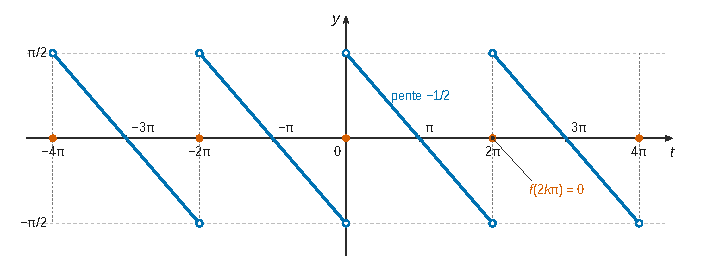
\includegraphics{figures/q1-dent-de-scie.pdf}
\caption*{Figure 1 --- Graphe de f entre −4π et 4π : dent de scie de pente −1/2,
extrémités exclues (cercles vides), f(2kπ) = 0 (points pleins)}
\end{figure}

Graphe sur \([-4\pi,4\pi]\) : quatre segments de pente \(-\frac12\), un par intervalle \(]2k\pi,2(k+1)\pi[\).

Chaque segment coupe l'axe en \((2k+1)\pi\). En chaque \(2k\pi\), la fonction saute de \(-\frac\pi2\) à \(\frac\pi2\) et vaut \(0\).

\begin{longtable}[]{@{}
  >{\raggedright\arraybackslash}p{(\columnwidth - 8\tabcolsep) * \real{0.2000}}
  >{\raggedright\arraybackslash}p{(\columnwidth - 8\tabcolsep) * \real{0.2000}}
  >{\raggedright\arraybackslash}p{(\columnwidth - 8\tabcolsep) * \real{0.2000}}
  >{\raggedright\arraybackslash}p{(\columnwidth - 8\tabcolsep) * \real{0.2000}}
  >{\raggedright\arraybackslash}p{(\columnwidth - 8\tabcolsep) * \real{0.2000}}@{}}
\toprule\noalign{}
\begin{minipage}[b]{\linewidth}\raggedright
Intervalle
\end{minipage} & \begin{minipage}[b]{\linewidth}\raggedright
Expression de \(f(t)\)
\end{minipage} & \begin{minipage}[b]{\linewidth}\raggedright
Limite à droite
\end{minipage} & \begin{minipage}[b]{\linewidth}\raggedright
Zéro
\end{minipage} & \begin{minipage}[b]{\linewidth}\raggedright
Limite à gauche
\end{minipage} \\
\midrule\noalign{}
\endhead
\bottomrule\noalign{}
\endlastfoot
\(]-4\pi,-2\pi[\) & \(-\frac{3\pi+t}{2}\) & \(\frac\pi2\) & \(-3\pi\) & \(-\frac\pi2\) \\
\(]-2\pi,0[\) & \(-\frac{\pi+t}{2}\) & \(\frac\pi2\) & \(-\pi\) & \(-\frac\pi2\) \\
\(]0,2\pi[\) & \(\frac{\pi-t}{2}\) & \(\frac\pi2\) & \(\pi\) & \(-\frac\pi2\) \\
\(]2\pi,4\pi[\) & \(\frac{3\pi-t}{2}\) & \(\frac\pi2\) & \(3\pi\) & \(-\frac\pi2\) \\
\end{longtable}

(« Limite à droite » : en la borne gauche de l'intervalle ; « limite à gauche » : en sa borne droite. En \(-4\pi,-2\pi,0,2\pi,4\pi\), \(f\) vaut \(0\).)

Le graphe est symétrique par rapport à l'origine : le segment de \(]-2\pi,0[\) est l'image de celui de \(]0,2\pi[\) par \(t\mapsto-t\), \(y\mapsto-y\), ce qui traduit l'imparité.

\textbf{Question 2.} Pour \(n\ge1\), \(t\mapsto f(t)\cos(nt)\) est impaire (produit d'une fonction impaire et d'une fonction paire) et continue par morceaux.

Son intégrale sur le segment symétrique \([-\pi,\pi]\) est donc nulle : \(a_n=0\).

Pour \(n=0\), \(f\) est elle-même impaire, donc \(a_0=\frac1{2\pi}\int_{-\pi}^{\pi}f=0\).

\equationajustee{\boxed{\forall n\in\mathbb{N},\ a_n=0.}}

\textbf{Question 3(a).} Soit \(n\ge1\). On intègre par parties avec \(u=x\) et \(v=-\frac{\cos(nx)}{n}\), fonctions \({\mathcal{C}}^1\) sur \([0,\pi]\) :

\equationajustee{\begin{aligned}
\int_0^\pi x\sin(nx)\,dx&=\Big[-\frac{x\cos(nx)}{n}\Big]_0^\pi+\frac1n\int_0^\pi\cos(nx)\,dx\\
&=-\frac{\pi(-1)^n}{n}+\frac1{n^2}\big[\sin(nx)\big]_0^\pi\\
&=-\frac{\pi(-1)^n}{n}.
\end{aligned}}

\equationajustee{\boxed{\int_0^\pi x\sin(nx)\,dx=-\frac{\pi(-1)^n}{n}.}}

\textbf{Question 3(b).} \(t\mapsto f(t)\sin(nt)\) est paire (produit de deux fonctions impaires), donc :

\equationajustee{\begin{aligned}
b_n&=\frac2\pi\int_0^\pi\frac{\pi-t}{2}\sin(nt)\,dt\\
&=\int_0^\pi\sin(nt)\,dt-\frac1\pi\int_0^\pi t\sin(nt)\,dt\\
&=\frac{1-(-1)^n}{n}+\frac{(-1)^n}{n}.
\end{aligned}}

\equationajustee{\boxed{\forall n\ge1,\ b_n=\frac1n.}}

\textbf{Question 4.} \emph{Théorème de Dirichlet.} Si \(g\) est \(2\pi\)-périodique et de classe \({\mathcal{C}}^1\) par morceaux sur \(\mathbb{R}\), sa série de Fourier converge en tout point \(t\).

Sa somme vaut alors \(\frac12\big(g(t^+)+g(t^-)\big)\) ; en particulier, elle vaut \(g(t)\) en tout point de continuité.

\emph{Hypothèses.} \(f\) est \(2\pi\)-périodique. Sur \(]0,2\pi[\), elle coïncide avec la fonction affine \(t\mapsto\frac{\pi-t}{2}\).

Cette fonction affine se prolonge en une fonction \({\mathcal{C}}^1\) sur \([0,2\pi]\) : \(f\) est donc \({\mathcal{C}}^1\) par morceaux.

\emph{Points de continuité.} \(f\) est continue sur \(\mathbb{R}\setminus2\pi\mathbb{Z}\), donc \(S(t)=f(t)\) en ces points.

\emph{Points de discontinuité.} En \(2k\pi\), la série converge vers la demi-somme des limites latérales :

\equationajustee{\begin{aligned}
\frac12\big(f(0^+)+f(0^-)\big)&=\frac12\Big(\frac\pi2-\frac\pi2\Big)\\
&=0\\
&=f(2k\pi).
\end{aligned}}

\equationajustee{\boxed{\text{La \text{série} de Fourier de } f \text{ converge en tout point et } \forall t\in\mathbb{R},\ S(t)=f(t).}}

Avec les questions 2 et 3 :

\equationajustee{\boxed{\forall t\in\mathbb{R},\ \sum_{k=1}^{+\infty}\frac{\sin(kt)}{k}=f(t).}}

\textbf{Question 5(a).} Si \(k=2p\) avec \(p\in{\mathbb{N}}^*\), alors \(\sin\big(\frac{k\pi}2\big)=\sin(p\pi)=0\).

Si \(k=2p+1\) avec \(p\in\mathbb{N}\), alors \(p=\frac{k-1}2\) et :

\equationajustee{\begin{aligned}
\sin\Big(\frac{k\pi}2\Big)&=\sin\Big(p\pi+\frac\pi2\Big)\\
&=\cos(p\pi)\\
&=(-1)^p.
\end{aligned}}

\equationajustee{\boxed{\sin\Big(\frac{k\pi}{2}\Big)=\begin{cases}(-1)^{\frac{k-1}{2}}&\text{si } k \text{ impair},\\ 0&\text{si } k \text{ pair}.\end{cases}}}

\textbf{Question 5(b).} On a \(\frac\pi2\in\,]0,\pi[\), point de continuité de \(f\). Par la question 4 :

\equationajustee{\begin{aligned}
S\Big(\frac\pi2\Big)&=f\Big(\frac\pi2\Big)\\
&=\frac{\pi-\pi/2}{2}\\
&=\frac\pi4.
\end{aligned}}

D'autre part \(S\big(\frac\pi2\big)=\sum_{k\ge1}\frac{\sin(k\pi/2)}{k}\). D'après 5(a), les termes d'indice pair sont nuls.

La somme partielle d'indice \(2P+1\) vaut donc \(\sum_{p=0}^{P}\frac{(-1)^p}{2p+1}\). C'est une suite extraite de la suite des sommes partielles, qui converge vers \(\frac\pi4\) : elle a la même limite.

\equationajustee{\boxed{\begin{aligned}
S\Big(\frac\pi2\Big)&=\frac\pi4,\\
\sum_{p=0}^{+\infty}\frac{(-1)^p}{2p+1}&=\frac\pi4.
\end{aligned}}}

\textbf{Question 6.} \emph{Identité de Parseval.} Si \(g\) est \(2\pi\)-périodique et continue par morceaux sur \(\mathbb{R}\), de coefficients \(a_0,a_n,b_n\) (convention ci-dessus), alors :

\equationajustee{\frac1{2\pi}\int_{-\pi}^{\pi}g(t)^2\,dt=a_0^2+\frac12\sum_{n=1}^{+\infty}\big(a_n^2+b_n^2\big).}

\(f\) est \(2\pi\)-périodique et continue par morceaux : l'identité s'applique. Comme \(f^2\) est paire :

\equationajustee{\begin{aligned}
\frac1{2\pi}\int_{-\pi}^{\pi}f^2&=\frac1\pi\int_0^\pi\frac{(\pi-t)^2}{4}\,dt\\
&=\frac1{4\pi}\Big[-\frac{(\pi-t)^3}{3}\Big]_0^\pi\\
&=\frac{\pi^2}{12}.
\end{aligned}}

Avec \(a_0=a_n=0\) et \(b_n=\frac1n\), le membre de droite vaut \(\frac12\sum_{n\ge1}\frac1{n^2}\). On obtient :

\equationajustee{\frac12\sum_{n=1}^{+\infty}\frac1{n^2}=\frac{\pi^2}{12}.}

\equationajustee{\boxed{\sum_{n=1}^{+\infty}\frac1{n^2}=\frac{\pi^2}6.}}

\textbf{Question 7(a).} La fonction renvoie \(\sum_{k=1}^n\frac1{k^2}\). Pour \(n=3\) :

\equationajustee{\begin{aligned}
f(3)&=1+\frac14+\frac19\\
&=\frac{36+9+4}{36}.
\end{aligned}}

\equationajustee{\boxed{f(3)=\frac{49}{36}.}}

\textbf{Question 7(b).} La somme partielle croît vers \(\frac{\pi^2}6\) (question 6). L'écart \(\frac{\pi^2}6-\sum_{k=1}^n\frac1{k^2}\) décroît donc vers \(0\), et la boucle s'arrête.

\begin{lstlisting}[language=Python]
from math import pi

def approx(eps):
    cible = pi**2 / 6
    n = 1
    S = 1.0                      # S = somme des 1/k^2 pour k = 1..n
    while abs(S - cible) > eps:
        n = n + 1
        S = S + 1 / (n * n)
    return n
\end{lstlisting}

Exemples : \texttt{approx(0.1)} renvoie \(10\), \texttt{approx(0.001)} renvoie \(1000\) (le reste est de l'ordre de \(\frac1n\)).

En flottants, la somme cesse de croître pour \(n\) de l'ordre de \(10^8\) : la fonction n'est utilisable que pour \(\varepsilon\) pas trop petit (de l'ordre de \(10^{-7}\) au mieux).

\hypertarget{partie-b-extremum-de-s_n}{%
\subsection{\texorpdfstring{Partie B --- Extremum de \(S_n\)}{Partie B --- Extremum de S\_n}}\label{partie-b-extremum-de-s_n}}

D'après la partie A, \(S_n(t)=\sum_{k=1}^n\frac{\sin(kt)}{k}\).

\textbf{Question 8.} \(S_n\) est une somme finie de fonctions dérivables sur \(\mathbb{R}\). Elle est donc dérivable, et sa dérivée est la somme des dérivées, avec \(\big(\frac{\sin(kt)}k\big)'=\cos(kt)\).

\equationajustee{\boxed{\forall t\in\mathbb{R},\ S_n'(t)=\sum_{k=1}^n\cos(kt).}}

\textbf{Question 9(a).} On a \(\cos(kt)=\operatorname{Re}(e^{ikt})\), et \(\operatorname{Re}\) est additive :

\equationajustee{\begin{aligned}
\sum_{k=1}^n\cos(kt)&=\sum_{k=1}^n\operatorname{Re}(e^{ikt})\\
&=\operatorname{Re}\Big(\sum_{k=1}^ne^{ikt}\Big).
\end{aligned}}

\textbf{Question 9(b).} Pour \(t\notin2\pi\mathbb{Z}\), \(e^{it}\neq1\). On utilise la somme géométrique et la factorisation par l'angle moitié :

\equationajustee{e^{i\alpha}-1=e^{i\alpha/2}\big(e^{i\alpha/2}-e^{-i\alpha/2}\big)=2i\,e^{i\alpha/2}\sin\frac\alpha2.}

On obtient :

\equationajustee{\begin{aligned}
\sum_{k=1}^ne^{ikt}&=e^{it}\,\frac{e^{int}-1}{e^{it}-1}\\
&=e^{it}\,\frac{e^{i\frac{nt}2}\cdot2i\sin\frac{nt}2}{e^{i\frac t2}\cdot2i\sin\frac t2}\\
&=e^{i(n+1)\frac t2}\,\frac{\sin\frac{nt}2}{\sin\frac t2}.
\end{aligned}}

La division est licite car \(\sin\frac t2\neq0\), puisque \(\frac t2\notin\pi\mathbb{Z}\). Avec 9(a) :

\equationajustee{\boxed{\sum_{k=1}^n\cos(kt)=\operatorname{Re}\Big(e^{i(n+1)\frac t2}\,\frac{\sin(\frac{nt}2)}{\sin(\frac t2)}\Big).}}

\textbf{Question 9(c).} Le quotient \(\frac{\sin(nt/2)}{\sin(t/2)}\) est réel : il sort de la partie réelle. De plus \(\operatorname{Re}\big(e^{i(n+1)t/2}\big)=\cos\frac{(n+1)t}2\).

\equationajustee{\boxed{\forall t\in\mathbb{R}\setminus2\pi\mathbb{Z},\ \sum_{k=1}^n\cos(kt)=\frac{\cos(\frac{(n+1)t}{2})\sin(\frac{nt}{2})}{\sin(\frac t2)}.}}

\textbf{Question 10(a).} On utilise \(\sin u=0\iff u\in\pi\mathbb{Z}\) :

\equationajustee{\begin{aligned}
\sin\frac{nt}2=0&\iff\exists m\in\mathbb{Z},\ \frac{nt}2=m\pi\\
&\iff\exists m\in\mathbb{Z},\ t=\frac{2m\pi}n.
\end{aligned}}

\textbf{Question 10(b).} On utilise \(\cos u=0\iff u\in\frac\pi2+\pi\mathbb{Z}\) :

\equationajustee{\begin{aligned}
\cos\frac{(n+1)t}2=0&\iff\exists m\in\mathbb{Z},\ \frac{(n+1)t}2=\frac\pi2+m\pi\\
&\iff\exists m\in\mathbb{Z},\ t=\frac{\pi(2m+1)}{n+1}.
\end{aligned}}

\textbf{Question 10(c).} \emph{Points de \(2\pi\mathbb{Z}\).} Par la question 8, \(S_n'(2j\pi)=\sum_{k=1}^n1=n\neq0\) : aucun n'est critique.

\emph{Points de \(\mathbb{R}\setminus2\pi\mathbb{Z}\).} Par 9(c), comme \(\sin\frac t2\neq0\), \(S_n'(t)=0\) si et seulement si \(\sin\frac{nt}2=0\) ou \(\cos\frac{(n+1)t}2=0\).

Il faut retirer des ensembles de 10(a) et 10(b) leurs éléments dans \(2\pi\mathbb{Z}\) :
- \(\frac{2m\pi}n\in2\pi\mathbb{Z}\iff\frac mn\in\mathbb{Z}\iff m\in n\mathbb{Z}\) ;
- \(\frac{\pi(2m+1)}{n+1}=2j\pi\) imposerait \(2m+1=2j(n+1)\), impair égal à pair : impossible.

\equationajustee{\boxed{\{t\in\mathbb{R}\mid S_n'(t)=0\}=\Big\{\frac{2m\pi}n\ \Big|\ m\in\mathbb{Z}\setminus n\mathbb{Z}\Big\}\cup\Big\{\frac{\pi(2m+1)}{n+1}\ \Big|\ m\in\mathbb{Z}\Big\}.}}

\textbf{Question 11.} \emph{Première famille.} \(0\le\frac{2m\pi}n<2\pi\iff0\le m<n\). La condition \(m\notin n\mathbb{Z}\) retire \(m=0\) seulement : \(1\le m\le n-1\).

\emph{Seconde famille.} Pour \(m\) entier :

\equationajustee{\begin{aligned}
0\le\frac{\pi(2m+1)}{n+1}<2\pi&\iff0\le2m+1<2n+2\\
&\iff-\frac12\le m<n+\frac12\\
&\iff0\le m\le n.
\end{aligned}}

\equationajustee{\boxed{\begin{aligned}
t_{1,m}&=\frac{2m\pi}n,\quad 1\le m\le n-1,\\
t_{2,m}&=\frac{\pi(2m+1)}{n+1},\quad 0\le m\le n.
\end{aligned}}}

Remarque : l'égalité \(\frac{2m}{n}=\frac{2m'+1}{n+1}\) donne \(2m(n+1)=n(2m'+1)\).

Comme \(n\) et \(n+1\) sont premiers entre eux, \(n\mid2m\) avec \(0<2m<2n\), donc \(2m=n\).

Les deux familles ne se rencontrent qu'en \(\pi\), lorsque \(n\) est pair (\(m=m'=\frac n2\)).

\textbf{Question 12.} Pour \(n=3\) : \(t_{1,1}=\frac{2\pi}3\) et \(t_{1,2}=\frac{4\pi}3\). Puis \(t_{2,m}=\frac{(2m+1)\pi}4\) pour \(m=0,1,2,3\).

\equationajustee{\boxed{\{t\in[0,2\pi[\ \mid S_3'(t)=0\}=\Big\{\frac{2\pi}3,\frac{4\pi}3,\frac\pi4,\frac{3\pi}4,\frac{5\pi}4,\frac{7\pi}4\Big\}.}}

\begin{figure}[H]
\centering
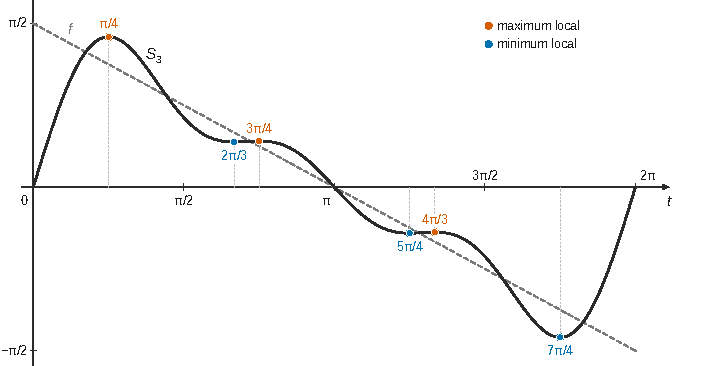
\includegraphics{figures/q12-s3-points-critiques.pdf}
\caption*{Figure 2 --- S₃ et ses six points critiques entre 0 et 2π : maxima
locaux en π/4, 3π/4, 4π/3, minima locaux en 2π/3, 5π/4, 7π/4 ; f en
tiretés}
\end{figure}

(La nature de chaque point, indiquée sur la figure, est établie aux questions 14 et 15.)

\textbf{Question 13(a).} On pose \(A=\frac{nt}2\) et \(B=\frac{(n+1)t}2\). Alors \(A+B=\big(n+\frac12\big)t\) et \(A-B=-\frac t2\), donc :

\equationajustee{2\cos\frac{(n+1)t}2\,\sin\frac{nt}2=\sin\Big(\Big(n+\frac12\Big)t\Big)-\sin\frac t2.}

On reporte dans 9(c), après avoir multiplié numérateur et dénominateur par \(2\) :

\equationajustee{\boxed{\forall t\in\mathbb{R}\setminus2\pi\mathbb{Z},\ S_n'(t)=\frac{\sin((n+\frac12)t)-\sin(\frac t2)}{2\sin(\frac t2)}.}}

\textbf{Question 13(b).} \(N\) et \(D\) sont dérivables, et \(D\) ne s'annule pas sur \(\mathbb{R}\setminus2\pi\mathbb{Z}\). Sur cet ensemble :

\equationajustee{S_n''=\frac{N'D-ND'}{D^2}.}

Si \(t\) est critique, \(\frac{N(t)}{D(t)}=0\), donc \(N(t)=0\), et :

\equationajustee{\begin{aligned}
S_n''(t)&=\frac{N'(t)D(t)}{D(t)^2}\\
&=\frac{N'(t)}{D(t)}.
\end{aligned}}

\equationajustee{\boxed{S_n''(t)=\frac{N'(t)}{D(t)}.}}

\textbf{Question 14(a).} (Le renvoi « question 6.(b) » de l'énoncé est lu comme 13.(b).) On dérive \(N\) :

\equationajustee{N'(t)=\Big(n+\frac12\Big)\cos\Big(\Big(n+\frac12\Big)t\Big)-\frac12\cos\frac t2.}

Pour \(t=t_{1,m}\) : \(\big(n+\frac12\big)t_{1,m}=2m\pi+\frac{m\pi}n\) et \(\frac{t_{1,m}}2=\frac{m\pi}n\). Par \(2\pi\)-périodicité du cosinus :

\equationajustee{\begin{aligned}
N'(t_{1,m})&=\Big(n+\frac12\Big)\cos\frac{m\pi}n-\frac12\cos\frac{m\pi}n\\
&=n\cos\frac{m\pi}n,\\
D(t_{1,m})&=2\sin\frac{m\pi}n.
\end{aligned}}

\(t_{1,m}\) est un point critique hors de \(2\pi\mathbb{Z}\), et 13(b) donne :

\equationajustee{\boxed{S_n''(t_{1,m})=\frac n2\,\frac{\cos(\frac{m\pi}n)}{\sin(\frac{m\pi}n)}.}}

\textbf{Question 14(b).} \(1\le m\le n-1\) donne \(\frac{m\pi}n\in\,]0,\pi[\), donc \(\sin\frac{m\pi}n>0\).

Le signe de \(S_n''(t_{1,m})\) est celui de \(\cos\frac{m\pi}n\). Ce cosinus est strictement positif si et seulement si \(\frac{m\pi}n<\frac\pi2\), c'est-à-dire \(m<\frac n2\), et strictement négatif si et seulement si \(m>\frac n2\).

\equationajustee{\boxed{\begin{aligned}
S_n''(t_{1,m})&>0 \text{ si } m<\tfrac n2,\\
S_n''(t_{1,m})&<0 \text{ si } m>\tfrac n2.
\end{aligned}}}

\textbf{Question 14(c).} En un point où \(S_n'\) s'annule et \(S_n''\neq0\), la formule de Taylor-Young à l'ordre 2 donne un minimum local strict si \(S_n''>0\), un maximum local strict si \(S_n''<0\).

\equationajustee{\boxed{t_{1,m}\ \text{est un minimum local si } m<\tfrac n2,\ \text{un maximum local si } m>\tfrac n2.}}

\textbf{Question 15(a).} On calcule :

\equationajustee{\begin{aligned}
\Big(n+\frac12\Big)t_{2,m}&=\frac{(2n+1)\pi(2m+1)}{2(n+1)}\\
&=\pi(2m+1)\,\frac{2(n+1)-1}{2(n+1)}\\
&=\pi(2m+1)-\frac{\pi(2m+1)}{2(n+1)}.
\end{aligned}}

Pour tout réel \(x\), on a \(\cos((2m+1)\pi)=-1\) et \(\sin((2m+1)\pi)=0\), donc :

\equationajustee{\begin{aligned}
\cos\big((2m+1)\pi-x\big)&=\cos((2m+1)\pi)\cos x+\sin((2m+1)\pi)\sin x\\
&=-\cos x.
\end{aligned}}

\equationajustee{\boxed{\cos\Big(\Big(n+\frac12\Big)t_{2,m}\Big)=-\cos\Big(\frac{\pi(2m+1)}{2(n+1)}\Big).}}

\textbf{Question 15(b).} Posons \(x_m=\frac{\pi(2m+1)}{2(n+1)}=\frac{t_{2,m}}2\). Par 15(a) :

\equationajustee{\begin{aligned}
N'(t_{2,m})&=-\Big(n+\frac12\Big)\cos x_m-\frac12\cos x_m\\
&=-(n+1)\cos x_m.
\end{aligned}}

\equationajustee{\boxed{N'(t_{2,m})=-(n+1)\cos\Big(\frac{\pi(2m+1)}{2(n+1)}\Big).}}

\textbf{Question 15(c).} \(t_{2,m}\notin2\pi\mathbb{Z}\) (question 10(c)) et \(D(t_{2,m})=2\sin x_m\). La question 13(b) donne :

\equationajustee{\boxed{S_n''(t_{2,m})=-\frac{n+1}2\,\frac{\cos(\frac{\pi(2m+1)}{2(n+1)})}{\sin(\frac{\pi(2m+1)}{2(n+1)})}.}}

\textbf{Question 15(d).} \(0\le m\le n\) donne \(1\le2m+1\le2n+1<2(n+1)\), donc \(x_m\in\,]0,\pi[\) et \(\sin x_m>0\).

Le signe de \(S_n''(t_{2,m})\) est l'opposé de celui de \(\cos x_m\). Or :

\equationajustee{\begin{aligned}
\cos x_m>0&\iff x_m<\frac\pi2\\
&\iff2m+1<n+1\\
&\iff m<\frac n2,
\end{aligned}}

et de même \(\cos x_m<0\iff m>\frac n2\).

\equationajustee{\boxed{\begin{aligned}
S_n''(t_{2,m})&<0 \text{ si } m<\tfrac n2,\\
S_n''(t_{2,m})&>0 \text{ si } m>\tfrac n2.
\end{aligned}}}

\textbf{Question 15(e).} Par le même critère qu'en 14(c) :

\equationajustee{\boxed{t_{2,m}\ \text{est un maximum local si } m<\tfrac n2,\ \text{un minimum local si } m>\tfrac n2.}}

Ainsi, sur \(]0,\pi[\), \(S_n\) présente successivement un maximum en \(t_{2,0}=\frac\pi{n+1}\), un minimum en \(t_{1,1}=\frac{2\pi}n\), un maximum en \(t_{2,1}\), etc.

\begin{center}\rule{0.5\linewidth}{0.5pt}\end{center}

\hypertarget{exercice-2}{%
\section{Exercice 2}\label{exercice-2}}

\(A=\begin{pmatrix}0&1&1\\1&0&1\\1&1&0\end{pmatrix}\).

\hypertarget{partie-a}{%
\subsection{Partie A}\label{partie-a}}

\textbf{Question 1(a).} On pose \(\chi_A(X)=\det(XI_3-A)\), polynôme de degré \(3\). On ajoute les deux dernières colonnes à la première, on factorise \(X-2\), puis on retranche la première ligne aux deux autres :

\equationajustee{\begin{aligned}
\chi_A(X)&=\begin{vmatrix}X&-1&-1\\-1&X&-1\\-1&-1&X\end{vmatrix}\\
&=(X-2)\begin{vmatrix}1&-1&-1\\1&X&-1\\1&-1&X\end{vmatrix}\\
&=(X-2)\begin{vmatrix}1&-1&-1\\0&X+1&0\\0&0&X+1\end{vmatrix}\\
&=(X-2)(X+1)^2.
\end{aligned}}

\equationajustee{\boxed{\chi_A(X)=X^3-3X-2=(X-2)(X+1)^2.}}

(Avec la convention \(\det(A-XI_3)\), on obtient l'opposé \(-X^3+3X+2\).)

\textbf{Question 1(b).} Les valeurs propres sont les racines de \(\chi_A\), lues sur la forme factorisée ; la multiplicité est l'exposant du facteur.

\equationajustee{\boxed{\begin{aligned}
\lambda_1&=-1\ \text{(\text{multiplicité} 2)},\\
\lambda_2&=2\ \text{(\text{multiplicité} 1)}.
\end{aligned}}}

\textbf{Question 2(a).} On résout \((A-2I_3)X=0\) :

\equationajustee{(x,y,z)\in E_2\iff\begin{cases}-2x+y+z=0\\x-2y+z=0\\x+y-2z=0\end{cases}}

La différence des deux premières équations donne \(x=y\), celle des deux dernières \(y=z\). Réciproquement, \(x=y=z\) vérifie le système.

\equationajustee{\boxed{\begin{aligned}
E_{\lambda_2}=E_2&=\operatorname{Vect}\big((1,1,1)^T\big),\\
\dim E_2&=1.
\end{aligned}}}

\textbf{Question 2(b).} \(A+I_3\) a ses trois lignes égales à \((1\ 1\ 1)\). Donc \((x,y,z)\in E_{-1}\iff x+y+z=0\) : c'est un plan vectoriel.

En écrivant \(x=-y-z\), on obtient \((x,y,z)=-y(1,-1,0)-z(1,0,-1)\), d'où une base :

\equationajustee{\boxed{\begin{aligned}
E_{\lambda_1}=E_{-1}&=\operatorname{Vect}\big((1,-1,0)^T,(1,0,-1)^T\big),\\
\dim E_{-1}&=2.
\end{aligned}}}

Les deux vecteurs sont dans \(E_{-1}\) et non colinéaires ; on retrouve \(\dim E_{-1}=3-\operatorname{rg}(A+I_3)=3-1=2\).

\textbf{Question 2(c).} La somme des dimensions des sous-espaces propres vaut \(\dim E_{-1}+\dim E_2=2+1=3\), la taille de la matrice. Donc \textbf{\(A\) est diagonalisable} :

\equationajustee{\begin{aligned}
P&=\begin{pmatrix}1&1&1\\-1&0&1\\0&-1&1\end{pmatrix},\\
D&=\begin{pmatrix}-1&0&0\\0&-1&0\\0&0&2\end{pmatrix},\\
A&=PDP^{-1}.
\end{aligned}}

\textbf{Question 3(a).} \(B-I_3\) a des \(0\) sur la diagonale et des \(1\) ailleurs : \(\boxed{A=B-I_3.}\)

\textbf{Question 3(b).} \(I_3\) commute avec toute matrice, donc \(B\) et \(I_3\) commutent, et \(B\) et \(-I_3\) aussi.

La formule du binôme de Newton s'applique donc dans \({\mathcal{M}}_3(\mathbb{R})\) : pour \(n\in\mathbb{N}\),

\equationajustee{\begin{aligned}
A^n&=(B+(-I_3))^n\\
&=\sum_{k=0}^n\binom nkB^k(-I_3)^{n-k},
\end{aligned}}

et \((-I_3)^{n-k}=(-1)^{n-k}I_3\).

\equationajustee{\boxed{A^n=\sum_{k=0}^n\binom nk(-1)^{n-k}B^k.}}

\textbf{Question 3(c).} Chaque coefficient de \(B^2\) vaut \(1\cdot1+1\cdot1+1\cdot1=3\) : \(B^2=3B\).

Montrons par récurrence sur \(k\ge1\) la propriété \(\mathcal{P}(k)\) : « \(B^k=3^{k-1}B\) ».

\emph{Initialisation.} Pour \(k=1\), \(B^1=B=3^0B\) : \(\mathcal{P}(1)\) est vraie.

\emph{Hérédité.} Soit \(k\ge1\) tel que \(\mathcal{P}(k)\) soit vraie. Alors :

\equationajustee{\begin{aligned}
B^{k+1}&=B^k\,B=3^{k-1}B^2\\
&=3^{k-1}\cdot3B=3^kB,
\end{aligned}}

donc \(\mathcal{P}(k+1)\) est vraie.

\emph{Conclusion.} Par récurrence, \(\mathcal{P}(k)\) est vraie pour tout \(k\ge1\).

\equationajustee{\boxed{\begin{aligned}
B^2&=3B,\\
\forall k\in{\mathbb{N}}^*,\ B^k&=3^{k-1}B.
\end{aligned}}}

\textbf{Question 3(d).} Pour \(n\ge1\), on isole le terme \(k=0\) de 3(b), égal à \((-1)^nI_3\) puisque \(B^0=I_3\). On applique 3(c) aux autres termes :

\equationajustee{\boxed{A^n=(-1)^nI_3+\Big(\sum_{k=1}^n\binom nk3^{k-1}(-1)^{n-k}\Big)B.}}

\textbf{Question 3(e).} Binôme dans \(\mathbb{R}\) :

\equationajustee{\begin{aligned}
\sum_{k=0}^n\binom nk3^k(-1)^{n-k}&=(3-1)^n\\
&=2^n.
\end{aligned}}

On retire le terme \(k=0\), égal à \((-1)^n\), puis on divise par \(3\) :

\equationajustee{\boxed{\sum_{k=1}^n\binom nk3^{k-1}(-1)^{n-k}=\frac13\big(2^n-(-1)^n\big).}}

\textbf{Question 3(f).} Pour \(n\ge1\), les questions 3(d) et 3(e) donnent :

\equationajustee{A^n=(-1)^nI_3+\frac{2^n-(-1)^n}3B.}

Les coefficients diagonaux valent \((-1)^n+\frac{2^n-(-1)^n}3\), les autres \(\frac{2^n-(-1)^n}3\).

Pour \(n=0\), les formules ci-dessous donnent \(a_0=1\) et \(b_0=0\), soit \(A^0=I_3\) : elles valent pour tout \(n\in\mathbb{N}\).

\equationajustee{\boxed{\begin{aligned}
A^n&=\begin{pmatrix}a_n&b_n&b_n\\b_n&a_n&b_n\\b_n&b_n&a_n\end{pmatrix},\\
a_n&=\frac{2^n+2(-1)^n}3,\\
b_n&=\frac{2^n-(-1)^n}3.
\end{aligned}}}

Contrôle : \(A^2=B^2-2B+I_3=B+I_3\), soit \(a_2=2\) et \(b_2=1\).

\hypertarget{partie-b}{%
\subsection{Partie B}\label{partie-b}}

\textbf{Question 4.} On calcule le produit ligne par ligne :

\equationajustee{\begin{aligned}
AX_n&=\begin{pmatrix}v_n+w_n\\u_n+w_n\\u_n+v_n\end{pmatrix}\\
&=\begin{pmatrix}u_{n+1}\\v_{n+1}\\w_{n+1}\end{pmatrix}.
\end{aligned}}

\equationajustee{\boxed{\forall n\in\mathbb{N},\ X_{n+1}=AX_n.}}

\textbf{Question 5.} Montrons par récurrence sur \(n\in\mathbb{N}\) la propriété « \(X_n=A^nX_0\) ».

\emph{Initialisation.} \(A^0X_0=I_3X_0=X_0\).

\emph{Hérédité.} Si \(X_n=A^nX_0\) pour un \(n\in\mathbb{N}\), alors, par la question 4, \(X_{n+1}=AX_n=A^{n+1}X_0\).

\emph{Conclusion.} La propriété est vraie pour tout \(n\in\mathbb{N}\).

\equationajustee{\boxed{\forall n\in\mathbb{N},\ X_n=A^nX_0.}}

\textbf{Question 6.} Avec 3(f), chaque ligne de \(A^n\) a pour somme \(a_n+2b_n\), donc :

\equationajustee{X_n=A^n\begin{pmatrix}1\\1\\1\end{pmatrix}=(a_n+2b_n)\begin{pmatrix}1\\1\\1\end{pmatrix}.}

Et :

\equationajustee{\begin{aligned}
a_n+2b_n&=\frac{2^n+2(-1)^n+2\cdot2^n-2(-1)^n}3\\
&=2^n.
\end{aligned}}

\equationajustee{\boxed{\begin{aligned}
X_n&=2^n\begin{pmatrix}1\\1\\1\end{pmatrix},\\
u_n=v_n=w_n&=2^n.
\end{aligned}}}

(Contrôle : \(X_0\) est vecteur propre de \(A\) pour la valeur propre \(2\), d'où \(A^nX_0=2^nX_0\).)

\begin{center}\rule{0.5\linewidth}{0.5pt}\end{center}

\hypertarget{exercice-3}{%
\section{Exercice 3}\label{exercice-3}}

\(\lambda\in\mathbb{C}\), \(|\lambda|=1\), \(\lambda\neq1\), \(f(z)=\lambda z\).

La suite est définie par \(z_{n+1}=\lambda z_n\) et \(z_0\in{\mathbb{C}}^*\).

\hypertarget{partie-a-uxe9tude-de-la-transformation}{%
\subsection{Partie A --- Étude de la transformation}\label{partie-a-uxe9tude-de-la-transformation}}

\textbf{Question 1.} Le module d'un produit est le produit des modules : \(|f(z)|=|\lambda|\,|z|=|z|\).

\textbf{Question 2.} On regroupe dans un membre :

\equationajustee{\begin{aligned}
f(z)=z&\iff(\lambda-1)z=0\\
&\iff z=0,
\end{aligned}}

car \(\lambda-1\neq0\). \(\boxed{\text{L'unique solution est } z=0.}\)

\textbf{Question 3.} Pour \(z\neq0\), on écrit \(z=|z|e^{i\varphi}\) avec \(\varphi=\arg z\). Alors :

\equationajustee{\begin{aligned}
f(z)&=e^{i\theta}\,|z|e^{i\varphi}\\
&=|z|e^{i(\varphi+\theta)},
\end{aligned}}

avec \(|z|>0\). C'est la forme exponentielle de \(f(z)\), donc :

\equationajustee{\boxed{\arg f(z)\equiv\arg z+\theta\pmod{2\pi}\qquad(z\neq0).}}

(\(z=0\) n'a pas d'argument.)

\textbf{Question 4.} \(D=\{r\mid r\in{\mathbb{R}}_+\}\), donc \(f(D)=\{r\lambda\mid r\ge0\}=\{re^{i\theta}\mid r\ge0\}\).

\equationajustee{\boxed{f(D)\ \text{est la demi-droite \text{fermée} d'origine } O \text{ \text{dirigée} par } e^{i\theta}.}}

\begin{figure}[H]
\centering
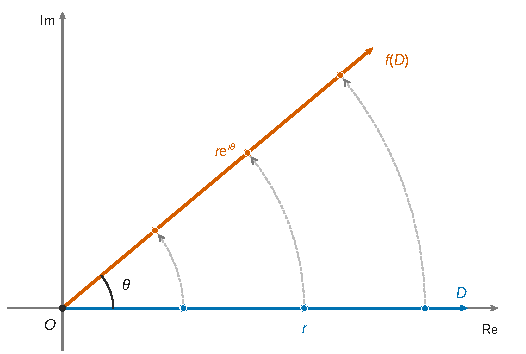
\includegraphics{figures/ex3-q4-image-demi-droite.pdf}
\caption*{Figure 3 --- Image de la demi-droite D par f : la demi-droite f(D)
d'origine O, tournée de θ ; chaque point r va en r·e\^{}(iθ)}
\end{figure}

Chaque point \(r\in D\) est envoyé sur le point de \(f(D)\) situé à la même distance \(r\) de \(O\).

Ainsi \(f\) est la rotation de centre \(O\) et d'angle \(\theta\).

\hypertarget{partie-b-uxe9tude-de-la-suite-z_n_ninmathbbn}{%
\subsection{\texorpdfstring{Partie B --- Étude de la suite \((z_n)_{n\in\mathbb{N}}\)}{Partie B --- Étude de la suite (z\_n)\_\{n\textbackslash in\textbackslash mathbb\{N\}\}}}\label{partie-b-uxe9tude-de-la-suite-z_n_ninmathbbn}}

\textbf{Question 5.} Montrons par récurrence sur \(n\in\mathbb{N}\) la propriété « \(z_n=\lambda^nz_0\) ».

\emph{Initialisation.} \(\lambda^0z_0=z_0\).

\emph{Hérédité.} Si \(z_n=\lambda^nz_0\) pour un \(n\in\mathbb{N}\), alors \(z_{n+1}=\lambda z_n=\lambda^{n+1}z_0\).

\emph{Conclusion.} \(\boxed{\forall n\in\mathbb{N},\ z_n=\lambda^nz_0.}\)

\textbf{Question 6.} \(|z_n|=|\lambda|^n|z_0|=|z_0|\).

\textbf{Question 7.} La distance de \(O\) au point d'affixe \(z_n\) est \(|z_n-0|=|z_0|\), avec \(|z_0|>0\).

\textbf{Le point d'affixe \(z_n\) appartient donc au cercle de centre \(O\) et de rayon \(|z_0|\).}

\textbf{Question 8(a).} On écrit \(\frac\theta{2\pi}=\frac ap\) avec \(a\in\mathbb{Z}\) et \(p\in{\mathbb{N}}^*\) (on choisit le dénominateur positif). Alors :

\equationajustee{\begin{aligned}
\lambda^p&=e^{ip\theta}\\
&=e^{2ia\pi}=1.
\end{aligned}}

\equationajustee{\boxed{\exists p\ge1,\ \lambda^p=1.}}

\textbf{Question 8(b).} Pour tout \(n\), \(z_{n+p}=\lambda^p\lambda^nz_0=z_n\).

\equationajustee{\boxed{(z_n) \text{ est \text{périodique}, de \text{période} } p.}}

\textbf{Question 9.} Supposons \((z_n)\) périodique de période \(p\ge1\), avec \(z_0\neq0\). Alors \(z_p=z_0\), soit \((\lambda^p-1)z_0=0\), donc \(\lambda^p=1\).

Ainsi \(e^{ip\theta}=1\) : il existe \(k\in\mathbb{Z}\) tel que \(p\theta=2k\pi\), et \(\frac\theta{2\pi}=\frac kp\in\mathbb{Q}\), ce qui contredit l'hypothèse.

\textbf{\((z_n)\) n'est pas périodique} (si \(z_0=0\), la suite serait nulle donc périodique).

\hypertarget{partie-c-application-numuxe9rique}{%
\subsection{Partie C --- Application numérique}\label{partie-c-application-numuxe9rique}}

\(z_0=1+i\), \(\lambda\in{\mathbb{U}}_N\).

\textbf{Question 10.} \(\boxed{r_0=|1+i|=\sqrt2}\), et \(z_0=\sqrt2\,e^{i\pi/4}\).

\textbf{Question 11.} On écrit \(\lambda=e^{i\theta}\), ce qui est possible car \(|\lambda|=1\). Alors \(\lambda^N=1\) s'écrit \(e^{iN\theta}=1\), soit \(N\theta\in2\pi\mathbb{Z}\).

\equationajustee{\boxed{\begin{aligned}
\lambda&=e^{\frac{2ik\pi}{N}}\\
&=\cos\frac{2k\pi}N+i\sin\frac{2k\pi}N,\quad k\in\{0,\dots,N-1\}.
\end{aligned}}}

L'hypothèse \(\lambda\neq1\) impose \(k\neq0\) (donc \(N\ge2\)). En particulier, \(\frac\theta{2\pi}=\frac kN\in\mathbb{Q}\).

\textbf{Question 12.} \(\lambda^N=1\), donc pour tout \(n\), \(z_{n+N}=\lambda^N\lambda^nz_0=z_n\).

\equationajustee{\boxed{(z_n) \text{ est \text{périodique}, } N \text{ est une \text{période}.}}}

(La plus petite période est \(\frac N{\gcd(k,N)}\).)

\begin{figure}[H]
\centering
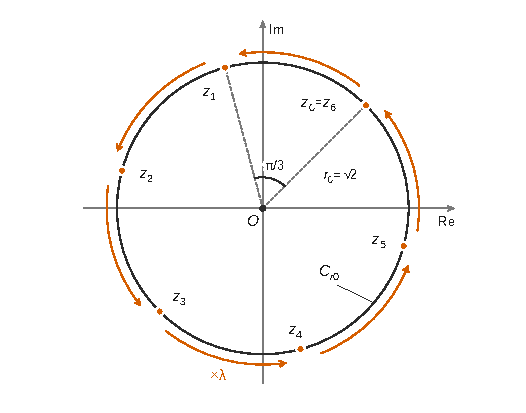
\includegraphics{figures/ex3-q12-orbite-periodique.pdf}
\caption*{Figure 4 --- Orbite de z₀ = 1 + i pour λ = e\^{}(iπ/3) dans U₆ : six
points sur le cercle de rayon r₀ = √2, chaque pas tourne de π/3, et z₆ =
z₀}
\end{figure}

\textbf{Question 13.} \emph{Inclusion directe.} Si \(\mu\in{\mathbb{U}}_N\), alors \((\lambda\mu)^N=\lambda^N\mu^N=1\), donc \(f({\mathbb{U}}_N)\subset{\mathbb{U}}_N\).

\emph{Inclusion réciproque.} Si \(\nu\in{\mathbb{U}}_N\), le complexe \(\mu=\lambda^{-1}\nu\) vérifie \(\mu^N=\frac{\nu^N}{\lambda^N}=1\) et \(f(\mu)=\nu\). Donc \({\mathbb{U}}_N\subset f({\mathbb{U}}_N)\).

\equationajustee{\boxed{f({\mathbb{U}}_N)={\mathbb{U}}_N.}}

\textbf{Question 14.} \(\lambda=e^{i\theta}\) avec \(\theta=2\sqrt2\pi\) ; on a \(|\lambda|=1\) et \(\lambda\neq1\).

De plus \(\frac\theta{2\pi}=\sqrt2\notin\mathbb{Q}\) : si \(\sqrt2=\frac ab\) sous forme irréductible, \(a^2=2b^2\) rend \(a\) pair, puis \(b\) pair.

Comme \(z_0=1+i\neq0\), la question 9 s'applique : \(\boxed{(z_n) \text{ n'est pas \text{périodique}.}}\)

\textbf{Question 15.} \emph{Existence.} Les \(z_n\) sont deux à deux distincts : \(z_n=z_m\) avec \(n<m\) donnerait \(\lambda^{m-n}=1\), donc \(\frac\theta{2\pi}\in\mathbb{Q}\).

Découpons \(C_{r_0}\) en \(K\) arcs de corde inférieure à \(\varepsilon\).

Parmi \(z_0,\dots,z_K\), deux points \(z_n,z_m\) (\(n<m\)) tombent dans le même arc. Avec \(q=m-n\ge1\) :

\equationajustee{0<r_0|\lambda^q-1|=|z_m-z_n|<\varepsilon.}

Les points \(z_{jq}=(\lambda^q)^jz_0\), \(j\in\mathbb{N}\), parcourent alors le cercle dans un sens fixé, par pas de corde \(r_0|\lambda^q-1|<\varepsilon\), et en font le tour.

Tout \(z\in C_{r_0}\) est donc à distance \(<\varepsilon\) de l'un d'eux. L'ensemble \(\{n\in\mathbb{N}\mid|z_n-z|<\varepsilon\}\) est non vide et admet un plus petit élément.

\emph{Algorithme} (\(\theta\) est passé en paramètre) :

\begin{lstlisting}[language=Python]
import cmath

def premier_indice(eps, z, theta):
    lam = cmath.exp(1j * theta)   # lambda = e^{i theta}
    n = 0
    zn = 1 + 1j                   # z_0
    while abs(zn - z) >= eps:
        n = n + 1
        zn = lam * zn             # z_{n} = lambda * z_{n-1}
    print(n)
    return n
\end{lstlisting}

La boucle s'arrête au premier \(n\) tel que \(|z_n-z|<\varepsilon\), qui est affiché.

\begin{center}\rule{0.5\linewidth}{0.5pt}\end{center}

\hypertarget{exercice-4}{%
\section{Exercice 4}\label{exercice-4}}

\hypertarget{partie-a-uxe9tude-de-la-convergence-de-la-suite-a_n_ninmathbbn}{%
\subsection{\texorpdfstring{Partie A --- Étude de la convergence de la suite \((a_n)_{n\in{\mathbb{N}}^*}\)}{Partie A --- Étude de la convergence de la suite (a\_n)\_\{n\textbackslash in\{\textbackslash mathbb\{N\}\}\^{}*\}}}\label{partie-a-uxe9tude-de-la-convergence-de-la-suite-a_n_ninmathbbn}}

\textbf{Question 1(a).} Pour tout \(n\ge1\), \(a_{n+1}-a_n=\frac1{(n+1)!}>0\).

\equationajustee{\boxed{(a_n) \text{ est strictement croissante.}}}

\textbf{Question 1(b).} Soit \(n\ge1\). Avec \((n+1)!=(n+1)\,n!\), on réduit au dénominateur commun \(n(n+1)^2n!\) :

\equationajustee{\begin{aligned}
b_{n+1}-b_n&=\frac1{(n+1)!}+\frac1{(n+1)(n+1)!}-\frac1{n\,n!}\\
&=\frac{n(n+1)+n-(n+1)^2}{n(n+1)^2\,n!}\\
&=\frac{-1}{n(n+1)^2\,n!}<0.
\end{aligned}}

\equationajustee{\boxed{(b_n) \text{ est strictement \text{décroissante}.}}}

\textbf{Question 1(c).} Les trois conditions de la définition sont vérifiées : \((a_n)\) est croissante, \((b_n)\) est décroissante, et \(b_n-a_n=\frac1{n\,n!}\to0\).

\equationajustee{\boxed{(a_n) \text{ et } (b_n) \text{ sont adjacentes.}}}

\textbf{Question 1(d).} Par le théorème des suites adjacentes, \((a_n)\) et \((b_n)\) convergent vers une même limite \(\ell\in\mathbb{R}\).

Les monotonies étant strictes, \(a_n<\ell<b_n\) pour tout \(n\ge1\).

\textbf{Question 2(a).} \(t\mapsto e^{-t}\) est décroissante, donc \(e^{-1}\le e^{-t}\le1\) sur \([0,1]\).

On multiplie par \(t^n\ge0\) et on intègre sur \([0,1]\) (croissance de l'intégrale, bornes dans l'ordre croissant), avec \(\int_0^1t^n\,dt=\frac1{n+1}\) :

\equationajustee{\boxed{\forall n\in\mathbb{N},\ \frac1{e(n+1)}\le f_n\le\frac1{n+1}.}}

\textbf{Question 2(b).} Par 2(a), \(0\le\frac{f_n}{n!}\le\frac1{(n+1)!}\), et \(\frac1{(n+1)!}\to0\).

Par encadrement, \(\frac{f_n}{n!}\to0\), donc \(\boxed{\varphi_n\to e.}\)

\textbf{Question 3(a).} \(f_0=\int_0^1e^{-t}\,dt=1-e^{-1}\). Puis :

\equationajustee{\begin{aligned}
\varphi_0&=e\big(1-(1-e^{-1})\big)\\
&=1.
\end{aligned}}

\equationajustee{\boxed{\begin{aligned}
f_0&=1-\frac1e,\\
\varphi_0&=1.
\end{aligned}}}

\textbf{Question 3(b).} On intègre par parties avec \(u=t^{n+1}\) et \(v=-e^{-t}\), fonctions \({\mathcal{C}}^1\) sur \([0,1]\) :

\equationajustee{\begin{aligned}
f_{n+1}&=\big[-t^{n+1}e^{-t}\big]_0^1+(n+1)\int_0^1t^ne^{-t}\,dt\\
&=-\frac1e+(n+1)f_n.
\end{aligned}}

\equationajustee{\boxed{f_{n+1}=(n+1)f_n-\frac1e.}}

\textbf{Question 3(c).} On divise 3(b) par \((n+1)!=(n+1)\,n!\) :

\equationajustee{\begin{aligned}
\frac{f_{n+1}}{(n+1)!}&=\frac{(n+1)f_n-e^{-1}}{(n+1)\,n!}\\
&=\frac{f_n}{n!}-\frac{e^{-1}}{(n+1)!}.
\end{aligned}}

On reporte dans la définition de \(\varphi_{n+1}\) :

\equationajustee{\begin{aligned}
\varphi_{n+1}&=e\Big(1-\frac{f_n}{n!}\Big)+\frac{e\cdot e^{-1}}{(n+1)!}\\
&=\varphi_n+\frac1{(n+1)!}.
\end{aligned}}

\equationajustee{\boxed{\varphi_{n+1}=\varphi_n+\frac1{(n+1)!}.}}

\textbf{Question 3(d).} Par définition, \(a_{n+1}=a_n+\frac1{(n+1)!}\).

(Lecture retenue de l'énoncé : « en déduire que, pour tout entier naturel non nul, \(\varphi_n=a_n\) ».) Montrons par récurrence sur \(n\ge1\) la propriété « \(\varphi_n=a_n\) ».

\emph{Initialisation.} Par 3(a) et 3(c), \(\varphi_1=\varphi_0+\frac1{1!}=2\), et \(a_1=1+1=2\).

\emph{Hérédité.} Si \(\varphi_n=a_n\) pour un \(n\ge1\), alors \(\varphi_{n+1}=a_n+\frac1{(n+1)!}=a_{n+1}\).

\emph{Conclusion.} \(\boxed{\forall n\ge1,\ \varphi_n=a_n.}\)

\textbf{Question 3(e).} \(a_n=\varphi_n\to e\) (question 2(b)). Par unicité de la limite :

\equationajustee{\boxed{\begin{aligned}
\ell&=e,\\
\sum_{k=0}^{+\infty}\frac1{k!}&=e.
\end{aligned}}}

\hypertarget{partie-b-uxe9tude-de-la-convergence-de-la-suite-c_n_ninmathbbn}{%
\subsection{\texorpdfstring{Partie B --- Étude de la convergence de la suite \((c_n)_{n\in{\mathbb{N}}^*}\)}{Partie B --- Étude de la convergence de la suite (c\_n)\_\{n\textbackslash in\{\textbackslash mathbb\{N\}\}\^{}*\}}}\label{partie-b-uxe9tude-de-la-convergence-de-la-suite-c_n_ninmathbbn}}

\textbf{Question 1.} \(c_n=e^{n\ln(1+1/n)}\). On pose \(x=\frac1n\), qui tend vers \(0\) : le développement limité de \(\ln(1+x)\) en \(0\) s'applique.

\equationajustee{\ln(1+x)=x-\frac{x^2}2+o(x^2).}

En multipliant par \(n\) :

\equationajustee{\begin{aligned}
n\ln\Big(1+\frac1n\Big)&=n\Big(\frac1n-\frac1{2n^2}+o\Big(\frac1{n^2}\Big)\Big)\\
&=1-\frac1{2n}+o\Big(\frac1n\Big).
\end{aligned}}

L'exposant tend vers \(1\), et non vers \(0\) : on ne peut pas composer directement avec le développement de l'exponentielle en \(0\).

On factorise donc \(e^1\) : \(c_n=e\cdot e^{u_n}\) avec \(u_n=-\frac1{2n}+o\big(\frac1n\big)\). Comme \(u_n\to0\), on peut utiliser \(e^u=1+u+o(u)\) au voisinage de \(0\) :

\equationajustee{\begin{aligned}
c_n&=e\cdot e^{u_n}\\
&=e\Big(1-\frac1{2n}+o\Big(\frac1n\Big)\Big).
\end{aligned}}

\equationajustee{\boxed{c_n=e-\frac e{2n}+o\Big(\frac1n\Big).}}

\textbf{Question 2.} \(\frac e{2n}\to0\) et \(o\big(\frac1n\big)\to0\) : \(\boxed{(c_n) \text{ converge vers } e.}\)

\hypertarget{partie-c-uxe9tude-de-la-vitesse-de-convergence-des-suites-a_n-et-c_n}{%
\subsection{\texorpdfstring{Partie C --- Étude de la vitesse de convergence des suites \((a_n)\) et \((c_n)\)}{Partie C --- Étude de la vitesse de convergence des suites (a\_n) et (c\_n)}}\label{partie-c-uxe9tude-de-la-vitesse-de-convergence-des-suites-a_n-et-c_n}}

\textbf{Question 1(a).} Par 1(d) et 3(e) de la partie A, \(a_{n+1}<e<b_n\). Donc :

\equationajustee{\begin{aligned}
e-a_n&<b_n-a_n=\frac1{n\,n!},\\
e-a_n&>a_{n+1}-a_n=\frac1{(n+1)!}.
\end{aligned}}

\equationajustee{\boxed{\forall n\ge1,\ \frac1{(n+1)!}\le e-a_n\le\frac1{n\cdot n!}.}}

\textbf{Question 1(b).} \(e-a_n>0\), donc \((a_n)\) ne prend pas la valeur \(e\).

On majore le numérateur par 1(a) au rang \(n+1\), et on minore le dénominateur par 1(a) au rang \(n\) :

\equationajustee{\begin{aligned}
0<\frac{|a_{n+1}-e|}{|a_n-e|}&=\frac{e-a_{n+1}}{e-a_n}\\
&\le\frac{1/\big((n+1)(n+1)!\big)}{1/(n+1)!}\\
&=\frac1{n+1}.
\end{aligned}}

Comme \(\frac1{n+1}\to0\), l'encadrement donne \(\beta=0\) : \(\boxed{\text{la convergence de } (a_n) \text{ vers } e \text{ est rapide.}}\)

\textbf{Question 2(a).} Par B.1, \(c_n-e=-\frac e{2n}+o\big(\frac1n\big)\), avec \(\frac e{2n}\neq0\) :

\equationajustee{\boxed{c_n-e\underset{n\to+\infty}{\sim}-\frac e{2n}.}}

\textbf{Question 2(b).} Pour \(x>0\), \(\ln(1+x)<x\) : la fonction \(x\mapsto x-\ln(1+x)\) est nulle en \(0\) et de dérivée \(\frac x{1+x}>0\).

Donc \(n\ln(1+\frac1n)<1\) et \(c_n<e\) pour tout \(n\ge1\) : \((c_n)\) ne prend pas la valeur \(e\).

Par 2(a), \(|c_n-e|\sim\frac e{2n}\) et \(|c_{n+1}-e|\sim\frac e{2(n+1)}\), donc :

\equationajustee{\begin{aligned}
\frac{|c_{n+1}-e|}{|c_n-e|}&\sim\frac{e/(2(n+1))}{e/(2n)}\\
&=\frac n{n+1}\to1.
\end{aligned}}

\(\beta=1\) : \(\boxed{\text{la convergence de } (c_n) \text{ vers } e \text{ est lente.}}\)

\end{document}
